
%%%%%%%%%%%%%%%%%%%%%%%%%%%%%%%%%%%%%%%%%%%%%%%%%%%%%%%%%%%%%%%%%%%%%%%%%%%%%%%%%%
\chapter{Technical Designs}
\label{v1ch:tech-designs}
 
 
 
\section{LBNF Project}
 
LBNF will provide facilities at Fermilab and at SURF to enable the scientific program of DUNE. These facilities are geographically separated into the Near Site Facilities, those to be constructed at Fermilab, and the Far Site Facilities, those to be constructed at SURF. %They are summarized in sections below.
 
\subsection{Near Site Facilities}
 
The scope of LBNF at Fermilab is provision of the beamline plus the conventional facilities (CF) for this beamline as well as for the DUNE near detector. The layout of these facilities is shown in Figure~\ref{fig:nearsite-topo}. The science requirements as determined by the DUNE
Collaboration drive the performance of the beamline and near detector, which then provide requirements for the components, space, and functions necessary to construct, install, and operate the beamline and near detector. ES\&H and facility operations requirements (i.e., \textit{programmatic} requirements) also provide input to the design.
 
\begin{cdrfigure}[Layout of LBNF Near Site]{nearsite-topo}{Layout of LBNF Near Site}
  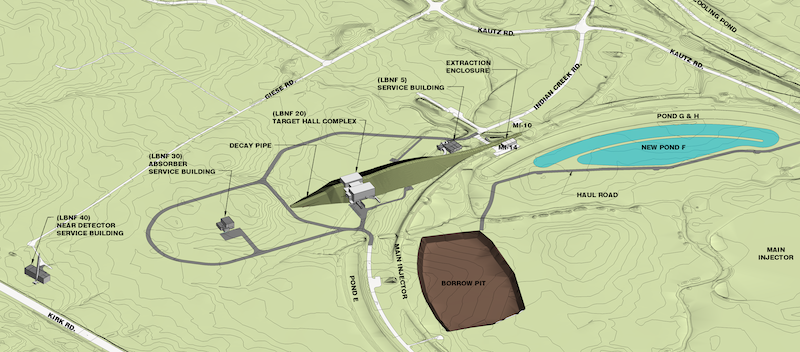
\includegraphics[width=\textwidth]{nearsite-topo}
\end{cdrfigure}
 
 
The beamline is designed to provide a neutrino beam of sufficient intensity and appropriate energy range to meet the goals of DUNE for long-baseline neutrino oscillation physics. The design is a conventional, horn-focused neutrino beamline. The components of the beamline will be designed to extract a proton beam from the Fermilab Main Injector (MI) and transport it to a target area where the collisions generate a beam of charged particles which decay into neutrinos to create the neutrino beam aimed at the near and far detectors.
 
The facility is designed for initial operation at proton-beam power of \SI{1.2}{\MW}, with the capability to support an upgrade to \SI{2.4}{\MW}. The plan is for twenty years of operation, while the lifetime of the Beamline Facility, including the shielding, is for thirty years. It is conservatively assumed that operations during the first five years will be at \MWadj{1.2} and the remaining fifteen years at \SI{2.4}{\MW}.  
The experience gained from the various neutrino projects has contributed extensively to the reference design. In particular, the NuMI beamline serves as the prototype design. Most of the subsystem designs and the integration between them follow, to a large degree, from previous projects. 
 
The proton beam will be extracted at a new point at MI-10. After extraction, this primary beam will establish a horizontally straight compass heading west-northwest toward the far detector, but will be bent upward to an apex before being bent downward at the appropriate angle. The primary beam is designed to be above grade to minimize expensive, underground construction; this also significantly enhances ground-water radiological protection. The design requires construction of an earthen embankment, or hill, whose dimensions are commensurate with the bending strength of the dipole magnets required for the beamline. 
 
The target marks the transition from the intense, narrowly directed proton beam to the more diffuse, secondary beam of particles that in turn decay to produce the neutrino beam. After collection and focusing, the pions and kaons that did not initially decay need a long, unobstructed volume in which to decay. This decay volume in the reference design is a pipe of circular cross section with its diameter and length optimized such that decays of the pions and kaons result in neutrinos in the energy range useful for the experiment. The decay volume is followed immediately by the absorber, which removes the remaining beam hadrons. 
 
Radiological protection is integrated into the LBNF beamline reference design in two important ways. First, shielding is optimized to reduce exposure of personnel to radiation dose and to minimize radioisotope production in ground water within the surrounding rock. Secondly, the handling and control of tritiated ground water produced in or near the beamline drives many aspects of the design. 
 
Beamline CF includes an enclosure connecting to the existing Main Injector at MI-10, concrete underground enclosures for the primary beam, targetry, horns, absorber, and related technical support systems. Service buildings will be constructed to provide support utilities the primary proton beam at LBNF~5 and to support the absorber at LBNF~30 (shown in Figure~\ref{fig:nearsite-topo}).  The Target Hall Complex at LBNF~20 houses the targetry system.  Utilities will be extended from nearby existing services, including power, domestic and industrial water, sewer, and communications. 
 
Near Detector CF includes a small muon alcove area in the Beamline Absorber Hall and a separate underground Near Detector Hall that houses the near detector. A service building called LBNF~40 with two shafts to the underground supports the near detector. The underground hall is sized for the reference near detector.
 
\subsection{Far Site Facilities}
 
The scope of LBNF at SURF includes both conventional facilities and cryogenic infrastructure to support the DUNE far detector. Figure~\ref{fig:lbnf-cavern-layout} shows the layout of the underground caverns that will house the detector modules with a separate cavern to house utilities and cryogenic systems. The requirements derive from DUNE Collaboration science requirements, which drive the space and functions necessary to construct and operate the far detector.  ES\&H and facility operations (programmatic) requirements also provide input to the design. The far detector is modularized into four \ktadj{10} fiducial mass detectors \fixme{determine if reference should be for total mass instead of fiducial}. The designs of the four detector pits in two caverns and the services to the caverns will be as similar to one another as possible for efficiency in design and construction as well as operation. 
 
\begin{cdrfigure}[LBNF Far Site cavern configuration]{lbnf-cavern-layout}{LBNF Far Site cavern configuration}  
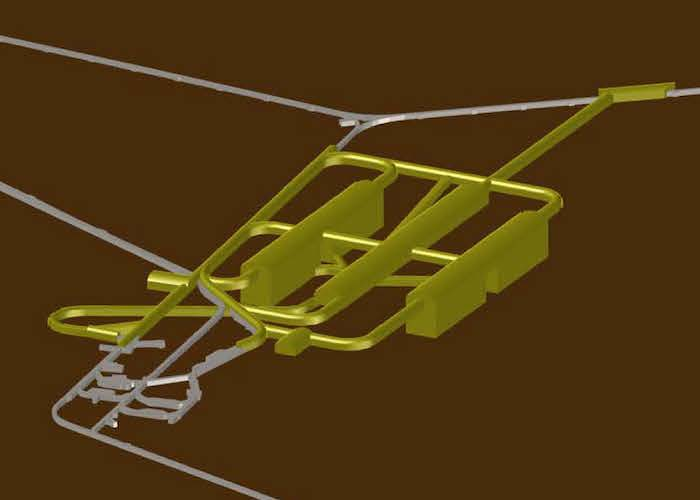
\includegraphics[width=.7\textwidth]{lbnf-cavern-layout}
\end{cdrfigure}
 
 
The scope of the Far Site CF includes design and construction for facilities both on the surface and underground. The underground conventional facilities includes new excavated spaces at the 4850L for the detector, utility spaces for experimental equipment, utility spaces for facility equipment, drifts for access, as well as construction-required spaces. Underground infrastructure provided by CF for the experiment includes power to experimental equipment, cooling systems and cyberinfrastructure. Underground infrastructure necessary for the facility includes domestic (potable) water, industrial water for process and fire suppression, fire detection and alarm, normal and standby power systems, a sump pump drainage system for native and leak water around the detector, water drainage to the facility-wide pump discharge system, and cyberinfrastructure for communications and security.
In addition to providing new spaces and infrastructure underground, CF will enlarge and provide infrastructure in some existing spaces for LBNF and DUNE use, such as the access drifts from the Ross Shaft to the new caverns. New piping will be provided in the shaft for cryogens (gas argon transfer line and the compressor suction and discharge lines) and domestic water as well as power conduits for normal and standby power and cyberinfrastructure. 
 
SURF currently has many surface buildings and utilities, some of which will be utilized for LBNF. The scope of the above-ground CF includes only that work necessary for LBNF, and not for the general rehabilitation of buildings on the site, which remains the responsibility of SURF. 
Electrical substations and distribution will be upgraded to increase power and provide standby capability for life safety. Additional surface scope includes a small control room in an existing building and a new building to support cryogen transfer from the surface to the underground near the existing Ross Shaft.
 
To reduce risk of essential but aging support equipment failure during the construction and installation period, several SURF infrastructure operations/maintenance activities are included as early activities in  the LBNF Project. These include completion of the Ross Shaft rehabilitation, rebuilding of hoist motors, and replacement of the Oro Hondo fan; if not addressed, this aging infrastructure could limit or remove access to the underground if equipment failed. 
 
The scope of the LBNF cryogenics infrastructure includes the design, fabrication, and installation of four cryostats to contain the liquid argon (LAr) and the detector components. It also includes a comprehensive cryogenic system that meets the performance requirements for purging, cooling and filling the cryostats, for achieving and maintaining the LAr temperature, and for purifying the LAr outside the cryostats. 
 
Each cryostat is composed of a free-standing steel-framed structure with a membrane cryostat vessel installed inside, to be constructed in one of the four excavated detector pits. The cryostat is designed to hold a total LAr mass capacity of 
17.1~kt. Each membrane tank cryostat has a stainless-steel liner as part of a full membrane system to provide full containment of the liquid cryogen. The hydrostatic pressure loading of the liquid cryogen is transmitted through rigid foam insulation to the surrounding structural steel frame which provides external support for the membrane. All penetrations into the interior of the cryostat will be made through the top plate to minimize the potential for leaks with the exception of the sidewall penetration for connection to the LAr recirculation system.
 
Cryogenic system components are located both on the surface and within the cavern. The cryogen receiving station is located on the surface near the Ross Shaft to allow for receipt of LAr deliveries for the initial filling period, as well as a buffer volume to accept liquid argon during the extended fill period. A large vaporizer for the nitrogen circuit feeds gas to one of four compressors located in the Cryogenic Compressor Building; the compressor discharges high pressure nitrogen gas to pipes in the Ross shaft. The compressors are located on the surface because the electrical power requirement and cooling requirement is much less than for similar equipment at the 4850L.  
 
Equipment at the 4850L includes the nitrogen refrigerator, liquid nitrogen vessels, argon condensers, external liquid argon recirculation pumps, and filtration equipment. Filling each cryostat with LAr in a reasonable period of time is a driving factor for the refrigerator and condenser sizing.  Each cryostat will have its own argon recondensers, argon-purifying equipment and overpressure protection system located in the Central Utility Cavern. Recirculation pumps will be placed outside and adjacent to each cryostat to circulate liquid from the bottom of the tank through the purifier.
 
 


\section{The DUNE Detectors}

The DUNE detectors to be installed at SURF (the far location) and FNAL (the near location) will enable the scientific program of DUNE.  The detector 
requirements derive from these DUNE science goals.

\subsection{The Far Detector}
The  Far Detector (FD) will be located deep underground at the 4850L and have
a  fiducial mass of \ktadj{40} to perform sensitive studies of long-baseline oscillations with a \kmadj{1300} baseline as well as a rich astroparticle physics programme and nucleon decay searches. The FD  will be composed of four %identical 
similar modules, each instrumented as a Liquid Argon Time Projection Chamber (LArTPC).
The concept of the LArTPC provides
excellent tracking and calorimetry performance, hence it is ideal for massive neutrino detectors such as DUNE's, which require a high signal efficiency and effective background discrimination,  an excellent capability to identify and  precisely measure neutrino events over a wide range of energies, and an excellent reconstruction of the kinematical properties
with a high resolution. The full imaging of events will allow study of neutrino interactions and
other rare events in an unprecedented way. \fixme{to an unprecedented level of precision?}
 The huge mass will allow collectiopn of sufficient statistics for precision
studies, as discussed in Chapter~\ref{v1ch:science}.

The LArTPC, pioneered in the context of the ICARUS project, is a mature technology. It is the outcome
of several decades of R\&D executed worldwide.  Nonetheless, the size of a single \ktadj{10} DUNE module represents an extrapolation by approximately one order of magnitude compared to the largest operated detector, the ICARUS~T600. To address this challenge, DUNE is developing two far detector options, the reference design and the alternative design, and is engaged in a 
comprehensive prototyping effort. At this stage, the development of two FD options is a strength and an added-value \fixme{asset or advantage?}
made possible by the merging of the worldwide neutrino community into DUNE.  The two detector
concepts are illustrated in Figure~\ref{fig:FarDet-overview-SPDP}.

\begin{cdrfigure}[3D models of the DUNE far detector designs]{FarDet-overview-SPDP}
{3D models of two 10-kt detectors using the single-phase reference design (left) 
and the dual-phase alternative design (right) for the DUNE far detector to be 
located at 4850L.}
\centering
\begin{minipage}[b]{1.0\textwidth}
\begin{center}
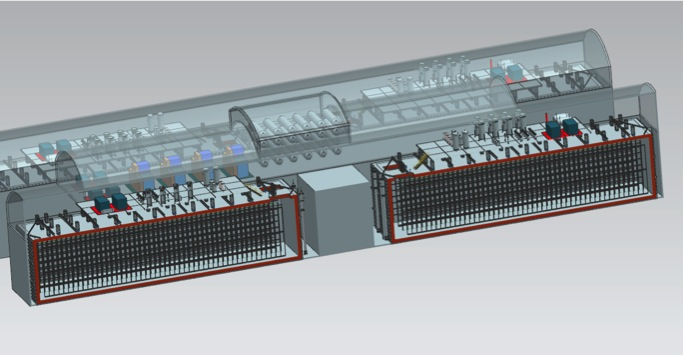
\includegraphics[width=.5\textwidth]{FarDet-3D-SP.jpg}
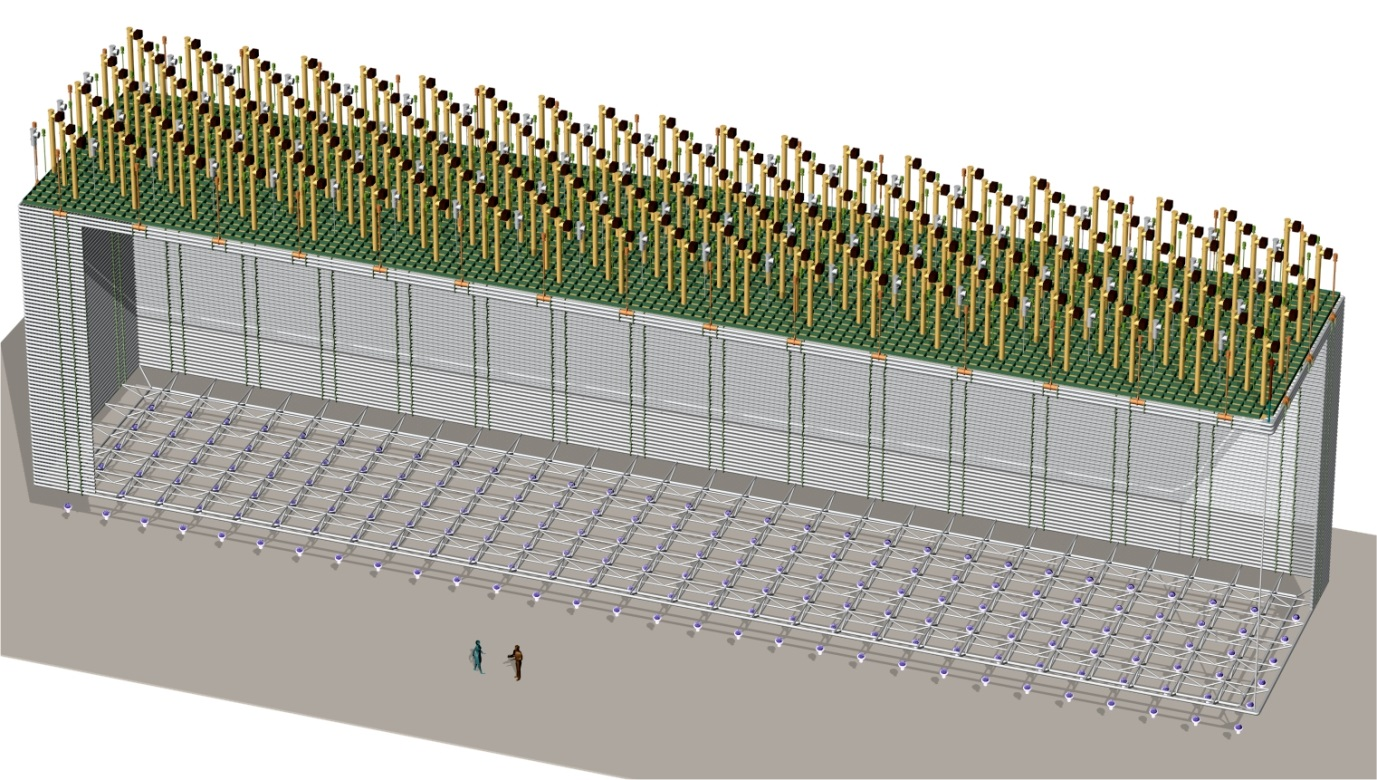
\includegraphics[width=0.46\textwidth]{DP_det2.jpg}
\end{center}
\end{minipage}
\end{cdrfigure}


Interactions in LAr produce ionization charge and scintillation light.
The charge is drifted with a constant electric field away from the cathode
plane and towards the segmented anode plane. \fixme{Maury had comments on this; I think it's that the negative charge, i.e., ionization electrons that are drifted away from cathode, not charge in general}
The prompt scintillation light,
detected by photo-detectors, provides the absolute time of the event.
The reference design adopts a single-phase readout, where the readout anode is composed wire planes in the LAr volume. 
In the alternative design, the  dual-phase approach is considered, in which the 
ionization charges are extracted, amplified and detected in gaseous argon (GAr) above the liquid surface. 
The dual-phase design would allow for a finer readout pitch (3~mm), 
a lower detection-energy threshold, and better pattern reconstruction of the events.
%The reference and alternative designs adopt complementary design to collect the scintillation light.
The photon-detection scheme used in both designs is similar. \fixme{Anne changed sentence}

The \ktadj{10} reference design TPC is described in Chapter 4 of \voldune. 
Its active volume is 12\,m high, 14.5\,m wide and 
58\,m long, instrumented with APAs, 
which are 6\,m high and 2.3\,m in width, and CPAs, 3\,m high by 2.5\,wide. Vertical stacks of
two APAs and four CPAs %are stacked vertically to 
instrument 
the 12\,m height of the active volume. The 12.5-m width of the detector is 
spanned by three stacks of APAs and two stacks of CPAs in an APA:CPA:APA:CPA:APA
arrangement, resulting in four 3.6\,m drift volumes, while the 58-m length of the active volume
is spanned by 25 such stack arrangements placed edge to edge. Hence a \ktadj{10} 
far detector module consists of 150 APAs and 200 CPAs. The CPAs are held a -180\,kV, such that 
ionization electrons drift a maximum distance of 3.6\,m in the electric field of 500\,V\,cm$^{-1}$.
The highly modular nature of the detector design allows for manufacturing to be distributed across a number of sites.

A  comprehensive prototyping strategy for both designs is actively pursued.
The reference design, closer to the original ICARUS design, is currently being validated in the 35-t prototype 
LAr detector at Fermilab.  The alternative design, representing a novel approach, has been proven on several
small-scale prototypes. Presently
a 20-t dual-phase prototype with dimensions 3$\times$1$\times$1~m$^3$ is being constructed at CERN (WA105),  
and should be operational in 2016. 
The ultimate validation of the engineered solutions for both designs of the FD is foreseen at 
the CERN Neutrino Platform around 2018, \fixme{is it a place or a program?} where full-scale engineering prototypes will be 
assembled and commissioned. Following this milestone, a test-beam data 
campaign will be executed %in the following years 
to collect a large sample of charged-particle interactions
in order to study the response of the detector with high precision.
A comprehensive list of synergies between the reference and alternative designs has been identified (Chapter 6 of \voldune). Common solutions for DAQ, electronics, HV feed-throughs, and so on, will pursued and implemented, independent of the details of the TPC design. The ongoing and planned efforts %and those at the CERN Neutrino Platform 
will
provide the ideal environment to exploit such synergies and implement common solutions.
There is recognition that the LArTPC technology will continue to evolve with (1) the large-scale prototypes at the CERN Neutrino Platform and the experience from the Fermilab SBN program, and (2) the experience gained during the construction and commissioning of the first \ktadj{10} module. 
The staged approach with the deployment of consecutive modules will
%give access to 
enable an early science program while allowing implementation of improvements and developments  during the experiment's lifetime.
The strategy for implementing
the far detector is presented in Chapter~\ref{v1ch:strategy}.

%%%%%%%%%%%%%%%%%%%%%%%%%%%%%%%%%%%%%%%%%%
\subsection{The Near Detector} %s} <--- I think there's only one overall near detector, right?

\fixme{We need to distinguish between near detector and near neutrino detector. I think the ND is NND+BLM+DAQ. Is this right?}

To meet the systematic precision needed to fulfill the DUNE science objectives, the near detector must thoroughly 
characterize the neutrino beam at the source, where it is composed of both muon- and electron-flavored neutrinos and antineutrinos. \fixme{Did I get this right?}  Additionally, it must precisely measure the cross sections and the particle yields of various processes that compose neutrino events.
 %
Its primary role is therefore collection of neutrino-interaction statistics to an uprecedented level. This wealth of fundamental neutrino-interaction 
measurements will satisfy important secondary scientific goals of the DUNE Collaboration. 
%
The reference design for the neutrino near detector (NND) design is the NOMAD-inspired fine-grained tracker (FGT), illustrated in Figure~\ref{fig:FGT_schematic}. The subsystems of the NND include a central 
straw-tube tracker and an electromagnetic calorimeter embedded in a 0.4-T dipole field. The steel of the
magnet yoke will be instrumented with muon identifiers. The strategy for implementation of
the Near Detector \fixme{ND or NND?} is presented in Chapter~\ref{v1ch:strategy}.

\fixme{The above is a rewrite of the following pgraph (so of course I propose dropping the following). Anne}
The spectrum and flavor composition of the neutrino beam will be measured with high precision 
in order to reach the ultimate sensitivity for the long-baseline neutrino oscillation studies.
The separation between fluxes of neutrinos and antineutrinos requires a magnetized neutrino detector to 
charge-discriminate electrons and muons produced in the neutrino charged-current interactions.
This is the primary role of the DUNE near detector system, however, being exposed to an intense flux of neutrinos
will also provides the opportunity to collect an unprecedentedly high statistics of neutrino 
interactions  for an extended science program. 
The near detector will therefore provide an opportunity for a wealth of fundamental neutrino interaction 
measurements, which are an important part of the secondary scientific goals of the DUNE collaboration. 
The reference design for the neutrino near detector (NND) design is the NOMAD-inspired fine-grained tracker (FGT), illustrated in Figure~\ref{fig:FGT_schematic}. The subsystems of NND comprise a central 
straw-tube tracker and an electromagnetic calorimeter embedded in a 0.4-T dipole field. The steel of the
magnet yoke will be instrumented with muon identifiers. The strategy to implement
the Near Detector is presented in Chapter~\ref{v1ch:strategy}.


\begin{cdrfigure}[A schematic drawing of the fine-grained
tracker design]{FGT_schematic}{A schematic drawing of the fine-grained tracker design}
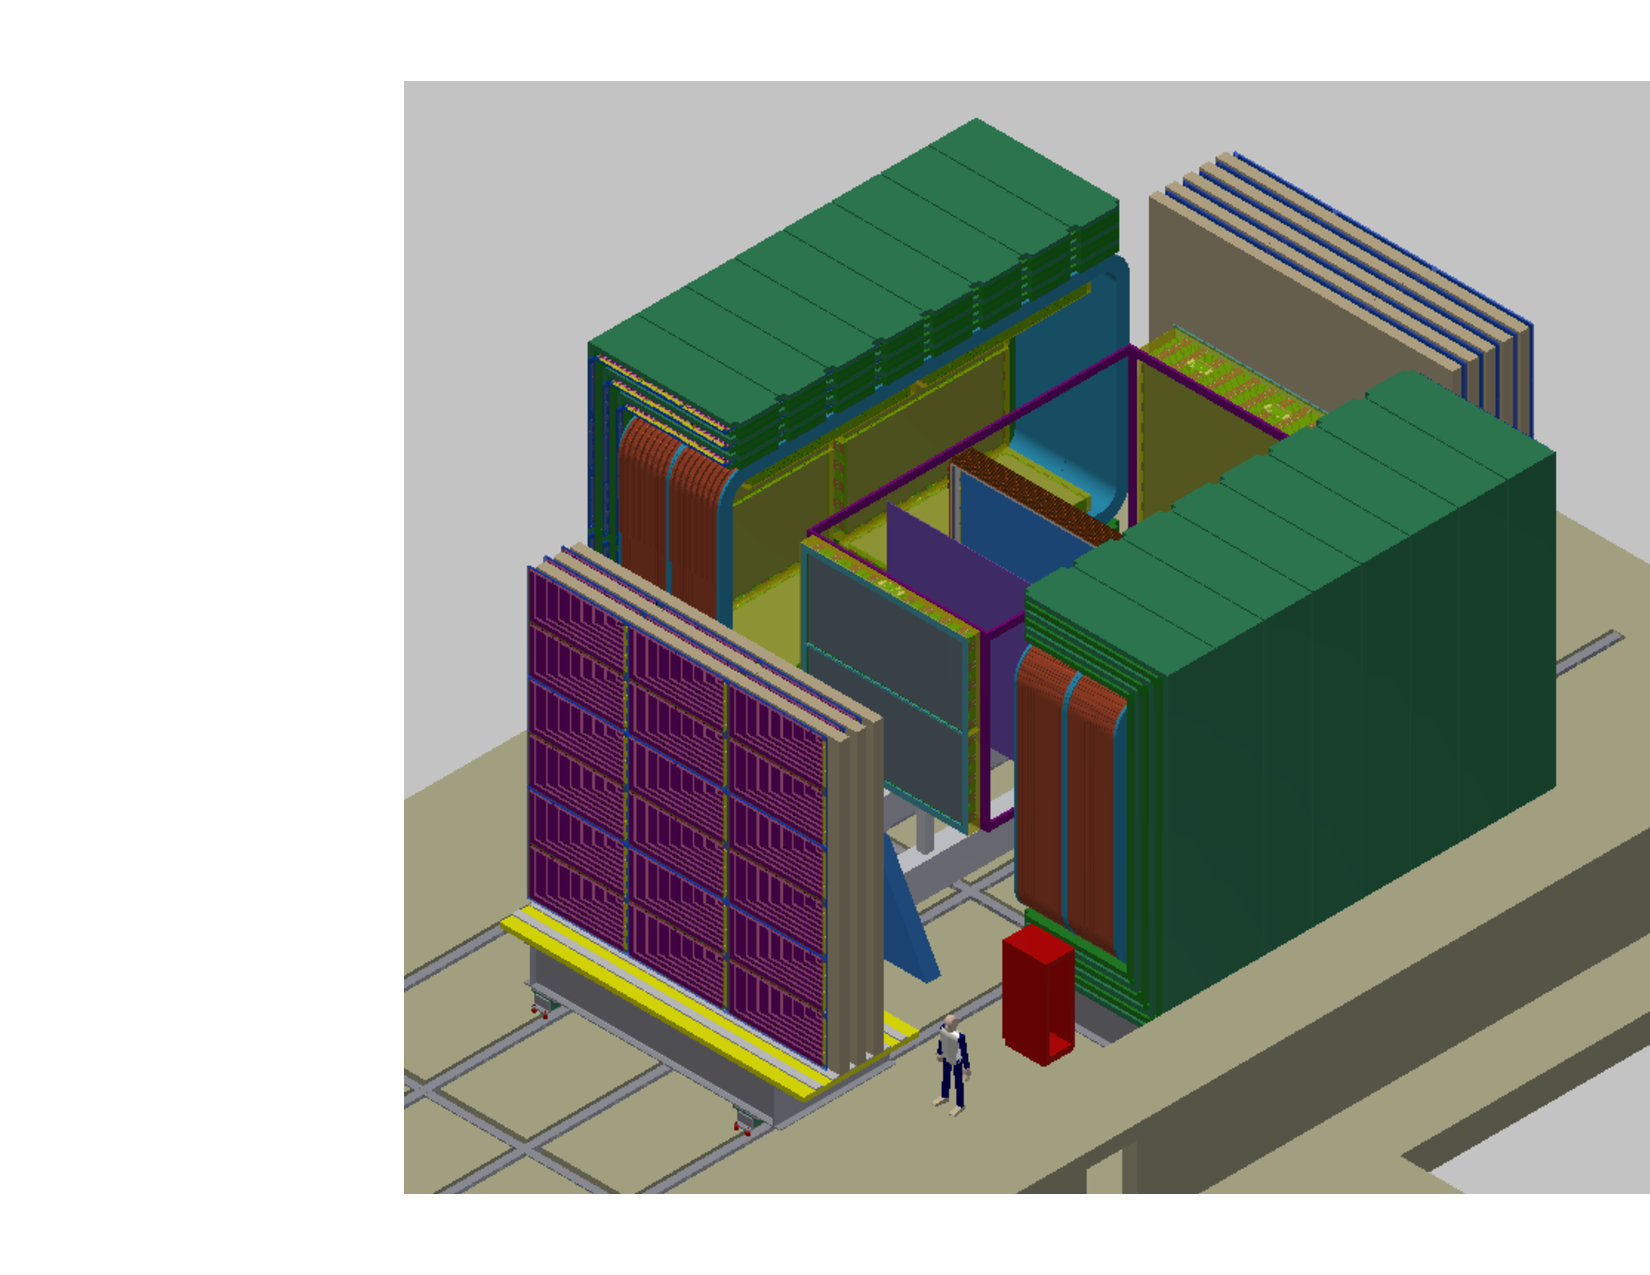
\includegraphics[width=.8\textwidth]{FGT_Overview}
\end{cdrfigure}


The NND will be complemented by a Beamline Measurement System (BLM) located in the region of the beam absorber at the downstream end of the decay region. The BLM aims to measure the muon fluxes from hadron decay and
 is intended to monitor the beam profile on a spill-by-spill basis. It will operate for the life of the experiment.


